\setchapterpreamble[u]{\margintoc}

\chapter{Grupos de homología singular}
\section{Símplices singulares}
Decimos que una familia de puntos $S=\{x_0, \dots, x_p\} \subset \mb{R}^n$ es \textbf{afínmente independiente} si, dados $\lambda_1,\dots,\lambda_n, \mu_1,\dots,\mu_n \in \mb{R}$ con
	\begin{align*}
		\sum^p_{i=0}\lambda_ix_i=\sum^p_{i=0}\mu_ix_i; && \sum^p_{i=0}\lambda_i=\sum^p_{i=0}\mu_i
	\end {align*}
se verifica que $\lambda_i=\mu_i$ para todo $1\leq i \leq n$.

\begin{proposition}
	La familia de puntos $S=\{x_0, \dots, x_p\} \subset \mb{R}^n$ es afínmente independiente si y sólo si la familia de vectores $\{x_1-x_0,\dots,x_p-x_0\}$ es linealmente independiente.
\end{proposition}

\begin{proof}
	Sea $S$ afínmente independiente y $\lambda_1,\dots, \lambda_p$ tales que
	\begin{equation}\label{CombLinNula}
		\sum^p_{i=1}\lambda_i(x_i-x_0)=0 \iff \sum^p_{i=1}\lambda_ix_i=x_0\sum^p_{i=1}\lambda_i
	\end{equation}
	Definimos $\lambda_0=-\lambda_1-\dots-\lambda_p$.
	Por construcción, $\lambda_0+\lambda_1+\dots+\lambda_p=\lambda_0-\lambda_0=0$.
	Aplicando la identidad \eqref{CombLinNula},
		\[0=\sum^p_{i=1}\lambda_i(x_i-x_0)=\sum^p_{i=1}\lambda_i x_i-x_0\sum^p_{i=1}\lambda_i=\sum^p_{i=0}\lambda_i x_i\]
	Dado que $S$ es una familia afínmente independiente, $\lambda_i=0$ para todo $i=1,\dots,n$.
	Por tanto, $T$ es linealmente independiente.
	Recíprocamente, sea $T$ linealmente independiente y $\mu_0,\alpha_0,\dots,\mu_p,\alpha_p \in \mb{R}$ tales que
	\begin{align*}
		\sum_{i=0}^p \mu_ix_i=\sum_{i=0}^p \alpha_ix_i; && \sum_{i=0}^p \mu_i=\sum_{i=0}^p \alpha_i
	\end{align*}
	Combinando ambas igualdades, deducimos que
	\begin{align*}
	0=\sum^p_{i=0}(\mu_i-\alpha_i)x_i
		&=\sum^p_{i=0}(\mu_i-\alpha_i)x_i-0x_0=\\
		&=\sum^p_{i=0}(\mu_i-\alpha_i)x_i-
		\left(\sum^p_{i=0}(\mu_i-\alpha_i)\right)x_0=\\
		&=\sum^p_{i=1}(\mu_i-\alpha_i)(x_i-x_0)
	\end{align*}
	Dado que $T$ es linealmente independiente, se sigue que
		\[\mu_i-\alpha_i=0 \iff \mu_i=\alpha_i\]
	para $i=1,\dots,p$.
	Por tanto, $S$ es afínmente independiente.
\end{proof}

\begin{marginfigure}
\begin{tikzpicture}[scale=0.6]
	%Puntos
	\draw (3,3)[fill=black] circle (1pt);
	\draw (3,3.5) node {$a$};

	\draw (0,0)[fill=black] circle (1pt);
	\draw (0,-.5) node {$b$};

	\draw (-3,3)[fill=black] circle (1pt);
	\draw (-3,3.5) node {$c$};

	%Vectores
	\draw[-to] (0,0) -- (1,1);
	\draw[-to] (0,0) -- (-1,1);

	%Líneas
	\draw[dashed] (-1,-1) -- (4,4);
	\draw (2,1.5) node {$L_1$};

	\draw[dashed] (1,-1) -- (-4,4);
	\draw (-2,1.5) node {$L_2$};
\end{tikzpicture}
\labfig{puntos independendientes}
\caption[Puntos afínmente independientes]{La independencia afín es el equivalente en conjuntos afines a la independencia lineal.}
\end{marginfigure}

Sea $S \subset \mb{R}^n$ afínmente independiente y $(a,b,c)$ una terna en $S$ con $a\neq b \neq c$.
Si $S$ es afínmente independiente, $a-b$ y $b-c$ son linealmente independientes.
Como $a-b\neq 0$, existen rectas afines $L_1,L_2 \subset \mb{R}^n$ que son paralelas a $a-b$ y $b-c$.
Por independencia lineal, $L_1$ y $L_2$ se cruzan a lo sumo en un punto, por lo que $a \not\in L_2$ y $c \not\in L_1$ (ver \reffig{puntos independientes}).

\begin{definition}
	Un \textbf{$p$-símplice} es la envoltura convexa de una familia afínmente independiente $\{x_0, \dots,x_p\} \subset \mb{R}^n$.
	Dichos puntos reciben el nombre de \textbf{vértices} del símplice.
\end{definition}

\marginnote{
\begin{kaobox}[frametitle=Envoluta convexa]
	Un $C \subseteq \mb{R}^n$ no vacío es convexo si, dados $x,y \in C$, $C$ contiene al segmento $[x,y]=\{xt+y(1-t)\colon t \in [0,1]\}$.
	Si $A \subset \mb{R}^n$ es no vacío, se define su \textbf{envoltura convexa} como el menor subconjunto convexo que contiene a $A$,
		\[\con(A)=\bigcup_{x,y \in A}[x,y]\]
\end{kaobox}
}

\begin{proposition}\labprop{BaseVertices}
	Sea $S\subset \mb{R}^n$ un $p$-símplice y $\{x_0,\dots x_p\}$ una familia afínmente independiente de puntos contenidos en $S$.
	Dado $x \in S$, existen únicos $t_0,\dots, t_p \in [0,1]$ tales que
	\begin{align*}
		x=\sum^p_{i=0}t_ix_i; && \sum^p_{i=0}t_i=1
	\end{align*}
\end{proposition}

Decimos que un $p$-símplice está \textbf{ordenado} cuando se aplica una relación de orden determinada sobre sus vértices.

\begin{example}
	Sean $a=(1,0,0)$, $b=(0,1,0)$ y $c=(0,0,1)$.
	La envoltura convexa de $\{a,b,c\}$ es un 2-símplice $\sigma$.
	Si $e_1=a$, $e_2=b$ y $e_3=c$, la relación de orden $e_i \leq e_j \leftrightharpoons i \leq j$ hace que $\sigma$ sea un 2-símplice ordenado.
\end{example}

\begin{marginfigure}
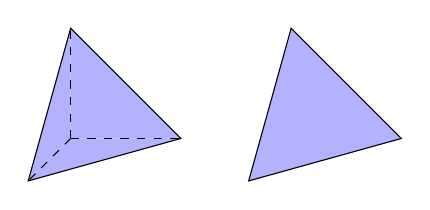
\begin{tikzpicture}[scale=1.4]
	% X: Left	/ Right
	% Y: Up		/ Down
	% Z: Front	/ Back

	% Tetrahedron
	\draw[fill=blue!30, draw opacity=0] (1,0,0) -- (0,1,0) -- (0,0,0) -- cycle;
	\draw[fill=blue!30, draw opacity=0] (1,0,0) -- (0,0,1) -- (0,0,0) -- cycle;
	\draw[fill=blue!30, draw opacity=0] (0,1,0) -- (0,0,1) -- (0,0,0) -- cycle;
	\draw[dashed] (0,0,0) -- (0,0,1);
	\draw[dashed] (0,0,0) -- (0,1,0);
	\draw[dashed] (0,0,0) -- (1,0,0);
	\draw (0,1,0) -- (0,0,1) -- (1,0,0) -- cycle;

	% Triangle
	\draw[fill=blue!30] (3,0,0) -- (2,0,1) -- (2,1,0) -- cycle;
\end{tikzpicture}
\caption[Triángulo y tetraedro]{Los triángulos y tetraedros constituyen ejemplos de símplices.
Se puede definir una teoría de homología equivalente a la homología singular utilizando sólo símplices, llamada \emph{homología simplicial} (véase \cite{Hatcher}).}
\labfig{123Simplice}
\end{marginfigure}

Sea $\{e_1, \dots, e_{n+1}\}$ la base canónica de $\mb{R}^{n+1}$.
La envoltura convexa de los puntos $\{e_1, \dots, e_{n+1}\}$ es un $n$-símplice, que denotaremos como $\sigma_n$.
Por \refprop{BaseVertices}, los puntos de $\sigma_n$ son de la forma
\begin{align*}
	(t_1,\dots,t_{n+1}) \in \mb{R}^{n+1}; && t_1+\dots+t_{n+1}=1
\end{align*}

Sea $S=\{x_0,\dots,x_n\}\subset \mb{R}^m$ una familia de puntos afínmente independientes: la aplicación continua
\begin{funcion*}
	f\colon \sigma_n \arrow[r]           & \con(S)            \\
	{(t_0,\dots,t_n)} \arrow[r, maps to] & \displaystyle\sum^n_{i=0}t_ix_i
\end{funcion*}
establece una biyección entre $\sigma_n$ y $\con(S)$.
Dado que $\sigma_n$ es compacto y $\con(S)$ es un espacio de Hausdorff, $f$ es un homeomorfismo \sidecite{IntroTopo}, por lo que $\con(S)$ es homeomorfo a $\sigma_n$.
De aquí se sigue que todo $p$-símplice de $\mb{R}^{p+1}$ es homeomorfo a $\sigma_p$, por lo que se conoce como \textbf{$p$-símplice estándar}.

\begin{example}
	\labexample{simplices low dimensions}
	Los símplices en bajas dimensiones son $\sigma_0=\{1\}$, $\sigma_1=[e_1,e_2]$, $\sigma_2$ (el triángulo) y $\sigma_3$ (el tetraedro).
\end{example}

\begin{definition}
	Un \textbf{$p$-símplice singular} en un espacio topológico $X$ es una aplicación continua $\phi\colon \sigma_p \to X$.
\end{definition}

\begin{example}\labexample{S1Complejo}
	Sea $\mb{D}$ la circunferencia unidad en $\mb{C}$.
	La aplicación
	\begin{funcion*}
		\phi\colon \sigma_1 \arrow[r]	& \mb{D}\\
		(t_0,t_1) \arrow[maps to,r] 	& e^{\pi i t_0}
	\end{funcion*}
	es un símplice singular que envía al $1$-símplice estándar en el hemisferio norte de $\mb{D}$ (ver \reffig{Circunferencia}).
	Notemos que $\phi(\sigma_1)$ no es un segmento desde el punto de vista geométrico porque está curvado, pero sí lo es desde un punto de vista topológico, ya que $\phi$ es un homeomorfismo y $\sigma_1$ es un segmento.
\end{example}

\begin{marginfigure}
	\resizebox{\textwidth}{!}{
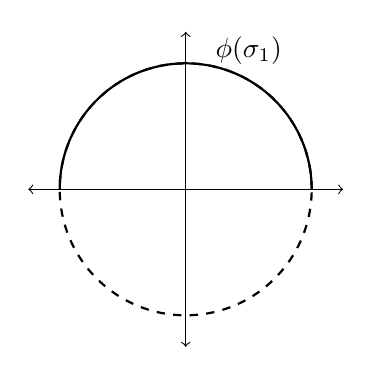
\begin{tikzpicture}[scale=0.8]
\draw [to-to] (-2.5,0) -- (2.5,0);
\draw [to-to] (0,-2.5) -- (0,2.5);

\draw[thick,dashed] (0,0) circle (2cm);

\draw[thick] (2,0) arc (0:180:2);
\draw (1,2.2) node {$\phi(\sigma_1)$};
\end{tikzpicture}
}
	\caption[Circunferencia]{La curva $\phi(\sigma_1)$ dada por el símplice singular $\phi$ de \refexample{S1Complejo}.
	Los símplices singulares amoldan el símplice estándar al espacio de llegada usando su continuidad.}
	\labfig{Circunferencia}
\end{marginfigure}

Dado un $p \in X$ y un espacio topológico $Y$, toda aplicación constante $\cte_p\colon Y \to X$ se identifica con el $0$-símplice singular $\phi_p\colon \sigma_0 \to X$ que envía al punto $1$ en $p$.
En general, todo camino $\alpha\colon [0,1] \to X$ se identifica con el $1$-símplice singular
\begin{funcion*}
\psi\colon	\sigma_1 \arrow[r]             & X      \\
		{(t_0,t_1)} \arrow[r, maps to] & \alpha(t_0)
\end{funcion*}

Sean $X$, $Y$ espacios topológicos.
Dada una aplicación continua $f\colon X \to Y$ y un $p$-símplice singular $\phi\colon \sigma_p \to X$, la aplicación $f_\#(\phi):=f\circ \phi\colon \sigma_p$ es un $p$-símplice singular en $Y$ por ser composición de aplicaciones continuas.
Esto hace que toda aplicación continua dé lugar a una aplicación que envía $p$-símplices singulares de $X$ en $p$-símplices singulares de $Y$.

\begin{proposition}\labprop{ComposicionAlmohadilla}
	\begin{enumerate}
	\item Si $\id$ es la identidad en $X$, $\id_\#$ es la identidad en $\sigma_n$;
	\item si $f\colon X \to Y$ y $g\colon Y \to Z$ son continuas, $(g\circ f)_\#=g_\#\circ f_\#$.
	\end{enumerate}
\end{proposition}

Sea $\phi\colon \sigma_p \to X$ un $p$-símplice singular y $0 \leq i \leq p$.
Se define la cara $i$-ésima de $\phi$ como el $(p-1)$-símplice singular
\begin{funcion*}
	\p_{(i)}\phi\colon \sigma_{p-1} \arrow[r] & X \\
	{(t_0,\dots,t_{p-1})} \arrow[r, maps to] & \phi(t_0,\dots,t_{i-1},0,t_{i},\dots,t_{p-1})
\end{funcion*}

\begin{example}
	El 2-símplice singular
	\begin{funcion*}
		\phi\colon  \sigma_2 \arrow[r] & \mb{R}^3 \\
		(x,y,z) \arrow[r, maps to] & (2x+2,2y+2,2z+2)
	\end{funcion*}
	tiene como caras
	\begin{align*}
		\p_{(0)}\phi(u,v)&=\phi(0,u,v)=(2,2u+2,2v+2)\\
		\p_{(1)}\phi(u,v)&=\phi(u,0,v)=(2u+2,2,2v+2)\\
		\p_{(2)}\phi(u,v)&=\phi(u,v,0)=(2u+2,2v+2,2)
	\end{align*}
	Desde un punto de vista geométrico, $\p_{(i)}\phi(\sigma_1)$ es una cara del tetraedro $\phi(\sigma_2)$.
\end{example}

\section{Grupos de homología}
Dado un grupo abeliano $G$, consideramos la acción $\rho\colon G\times \mb{Z} \to G$ dada por
\begin{align*}
	ng:=g+\stackrel{(n)}{\dots}+g	&& ng:=-g-\stackrel{(n)}{\dots}-g\\
	(n > 0)							&& (n < 0)
\end{align*}
Decimos que un subconjunto $S \subset G$ es un \textbf{sistema generador} de $G$ si, dado un $g \in G$, podemos hallar $b_1,\dots,b_n \in S$ y enteros $\mu_1,\dots,\mu_n$ tales que
\[g=\mu_1b_1+\mu_2b_2+\dots+\mu_nb_n\]

\begin{definition}
	Sea $G$ un grupo abeliano.
	Un sistema generador $B$ de $G$ es una \textbf{base} si, dados $b_1,\dots,b_n \in B$ y enteros $\lambda_1,\dots,\lambda_n$,
	\begin{equation}
		\label{SisLibre} \sum^n_{i=1}\lambda_ib_i=0 \implies \lambda_i=0
	\end{equation}
	Decimos que $G$ es un \textbf{grupo libre} si admite una base.
\end{definition}

\begin{example}
	Supongamos que el grupo aditivo $\mb{Q}$ es un grupo libre generado por un cierto conjunto $B \subseteq \mb{Q}$.
	Dados $\frac{a}{b}, \frac{c}{d} \in B$,
		\[cb\frac{a}{b}-ad\frac{c}{d}=0,\]
	por lo que $B$ está formado por un único elemento.
	Sea $p$ un número primo coprimo con $b$.
	Por ser $\mb{Q}$ libre, existirá un entero $\alpha$ tal que
		\[\frac{1}{p}=\alpha\frac{a}{b}\]
	pero esto implica que $b=\alpha pa$, en contradicción con la primalidad de $p$.
	Por tanto, $\mb{Q}$ no es un grupo libre.
\end{example}

\marginnote[-2.2cm]{
\begin{kaobox}[frametitle=Soporte de una aplicación]
	Dado un grupo abeliano $G$, el soporte de una aplicación $f\colon A \to G$ es el conjunto de los puntos donde no se anula.
\end{kaobox}
}

Se define el \textbf{grupo libre} generado por $A$ como la familia $\mc{F}(A)$ de todas las aplicaciones $f\colon A \to \mb{Z}$ con soporte finito, dotado con la suma de aplicaciones.

\begin{proposition}
	El grupo $\mc{F}(A)$ es libre.
\end{proposition}

\begin{proof}
	Dado un $a \in A$, denotamos $\mc{X}_a$ como la aplicación característica del conjunto $\{a\}$.
	Claramente, $\mc{X}_a \in \mc{F}(A)$.
	También denotamos $\mc{X}$ como la familia de todos los $\mc{X}_a$ con $a \in A$.

	Dada $f \in \mc{F}(A)$, se define $\tilde{f}$ como
		\[\tilde{f}=\sum_{a \in A}f(a)\mc{X}_a\]
	Dado un $x \in A$, $\tilde f(x)=f(x)$, por lo que $\mc{X}$ es un sistema generador de $\mc{F}(A)$.
	
	Sean $\mu_1,\dots,\mu_n$ enteros y $a_1,\dots,a_n \in A$ tales que $\mu_1\mc{X}_{a_1}+\dots+\mu_n\mc{X}_{a_n}=0$.
	Dado un $1 \leq j \leq n$,
		\[0=\sum^n_{i=1}\mu_i\mc{X}_{a_i}(a_j)=\mu_j\mc{X}_{a_j}(a_j)=\mu_j\]
	por lo que $\mu_1,\dots,\mu_n=0$ y $\mc{X}$ es una base.
\end{proof}

\begin{remark}
	Dado un conjunto finito $A$, $\mc{F}(A)\cong \mb{Z}^{|A|}$.
\end{remark}

\begin{definition}
	Un \textbf{grupo graduado} es una colección de grupos $G=\{G_n: n \in \mb{Z}\}$.
	Un grupo graduado $H$ es subgrupo graduado (resp. normal) de $G$ si $H_j \subseteq G_j$ (resp. $H_j \trianglelefteq G_j$) para todo $j$.
	Si $H$ es un subgrupo graduado normal de $G$, definimos
		\[\frac{G}{H}:=\left\{\frac{G_i}{H_i}: i \in \mb{Z}\right\}\]
\end{definition}

Sean $G,H$ grupos graduados.
Un \textbf{homomorfismo graduado} $f\colon G \to H$ es una colección de homomorfismos $f_i\colon G_i \to H_{i+r}$, donde $r \in \mb{Z}$ es un valor común para todos los $f_i$, llamado \emph{grado} de $f$.
Diremos que $f$ es un monomorfismo (resp. epimorfismo, isomorfismo, endomorfismo, automorfismo) graduado si lo es cada uno de los homomorfismos en la colección.

\begin{definition}
	Un \textbf{complejo de cadenas} es un par de la forma $(G,\p)$, siendo $G$ un grupo graduado y $\p$ un endomorfismo de grado $-1$ tal que
		\[\im  \p_n \leq \ker \p_{n-1}\]
	La aplicación $\p$ recibe el nombre de \textbf{operador borde}.
\end{definition}

\begin{definition}
Sean $(C,d)$ y $(C',d')$ dos complejos de cadenas.
Una \textbf{aplicación de cadenas} es un homomorfismo graduado $\Phi\colon C \to C'$ de grado $0$ tal que el siguiente diagrama es conmutativo:
	\begin{diagram*}
	C_{n+1} \arrow{r}{d_{n+1}} \arrow{d}{\Phi_{n+1}} & C_n \arrow{d}{\Phi_n} \\
	C'_{n+1} \arrow{r}{d'_{n+1}}                     & C'_n                   
	\end{diagram*}
\end{definition}

Sea $(C,d)$ un complejo de cadenas.
Se definen los grupos graduados
	\begin{align*}
		Z_*(C)&:=\ker d=\{\ker d_n: n \in \mb{Z}\};	& Z_n(C)&:=\ker d_n\\[0.2cm]
		B_*(C)&:=\im d=\{\im d_n: n \in \mb{Z}\}; 	& B_n(C)&:=\im d_n
	\end{align*}
Diremos que dos elementos $p,q \in Z_n(C)$ son \textbf{homólogos} si $p-q \in B_n(C)$.

\begin{definition}
	Se define el \textbf{grupo graduado de homología} $C$ como 
		\begin{align*}
			H_*(C):=\frac{Z_*(C)}{B_*(C)}
		\end{align*}
	Diremos que dos complejos de cadenas tienen el mismo \textbf{tipo de homología} si sus grupos de homología son isomorfos.
\end{definition}

Sea $f\colon (C,d) \to (D,\p)$ una aplicación de cadenas.
Dado un $c \in Z_n(C)$,
	\[d_n(c)=0 \implies \p_n[f_n(c)]=f_{n-1}[d_n(c)]=f_{n-1}(0)\]
Como $f_{n-1}$ es un homomorfismo de grupos, $f_{n-1}(0)=0$, por lo que $f_n(c)\in Z_n(D)$ y $f_n[Z_n(C)]\leq Z_n(D)$.
Análogamente, $f_n(B_n(C)) \leq B_n(D)$.
Por tanto, $f$ induce un homomorfismo entre grupos de homología,
	\[f_*\colon H_*(C) \to H_*(D)\]

\subsection{Homología de un espacio topológico}
\begin{definition}
	Se define el grupo de \textbf{$n$-cadenas singulares} $S_n(X)$ como el grupo libre generado por todos los símplices singulares $\phi\colon \sigma_n \to X$.
	Los elementos de $S_n(X)$ reciben el nombre de $n$-\emph{cadenas singulares} de $X$.
\end{definition}

A partir los grupos de cadenas singulares, podemos definir el grupo graduado
	\[S_*(X)=\{S_n(X): n \geq 0\}\]
Para poder completar el grupo graduado, simplemente se considera que $S_p(X)=0$ para todo $p < 0$.

El objetivo de esta sección es definir un operador borde sobre $S_*(X)$, de forma que $(S_*(X),\p)$ forme una complejo de cadenas.
Podemos extender el operador cara a $S_n(X)$ tomando
	\[\p_{(j)}\left(\sum_{i=1}^n k_i\phi_i\right)= \sum^n_{i=1}k_i\,\p_{(j)}\phi_i\]
Este proceso da lugar a $n+1$ operadores cara diferentes, pero ninguno de ellos define un operador borde.

\begin{definition}
	Se define el \textbf{operador borde} $\p\colon S_n(X) \to S_{n-1}(X)$ asociado a $S_*(X)$ como
		\[\p=\p_{(0)}-\p_{(1)}+\dots+(-1)^n\p_{(n)}\]
\end{definition}

\begin{theorem}\labthm{OperadorBorde}
Dado un espacio topológico $X$, $\im \p \leq \ker \p$.
Esto implica que $(S_*(X), \p)$ es un complejo de cadenas.
\end{theorem}

\begin{proof}
Sea $c \in S_n(X)$.
Dado que $S_n(X)$ es un grupo libre y $\p$ es un homomorfismo, podemos suponer sin pérdida de generalidad que $c$ es un símplice singular $\sigma_n \to X$.

Dados $0 \leq p, q \leq n$ con $p < q-1$,
\begin{align*}
\p_{(p)}\p_{(q)}&c(t_0,\dots,t_{n-2})
	=\p_{(q)}c(t_0,\dots,t_{p-1},\hat t_p,t_p,\dots,t_{n-2})=\\
	&=c(t_0,\dots,t_{p-1},\hat t_p,t_p,\dots,t_{q-2},\hat t_q,t_{q-1},\dots,t_{n-2})=\\
	&=\p_{(p)}c(t_0,\dots,t_{q-2},\hat t_{q-1},t_{q-1},\dots,t_{n-2})=\\
	&=\p_{(q-1)}\p_{(p)}c(t_0,\dots,t_{n-2})
\end{align*}
donde $\hat t$ denota reemplazar $t$ con un cero.
Por otro lado,
\begin{equation}
	\label{Borde2c}
	\p^2c=\sum^{n-1}_{p=0}(-1)^p\p_{(p)}(\p c)=\sum^n_{q=0}\sum^{n-1}_{p=0}(-1)^{p+q}\p_{(p)}\p_{(q)}c
\end{equation}

Combinando ambas expresiones,
	\[\p^2c=\sum_{q=1}^n\sum_{p < q-1}(-1)^{p+q}\p_{(p)}\p_{(q)}c+\sum^n_{q=0}\sum_{p > q}(-1)^{p+q}\p_{(p)}\p_{(q)}c\]
\begin{marginfigure}
	\resizebox{\textwidth}{!}{
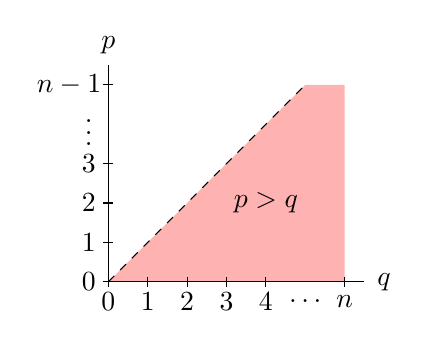
\begin{tikzpicture}[scale=.5]
%Región p > q
\filldraw[draw opacity=0, fill=red!30] (0,0) -- (5,5) -- (6,5) -- (6,0) -- cycle;
\draw[dashed] (0,0) -- (5,5);

\draw (0,5.5) -- (0,0) -- (6.5,0);
\draw (7,0) node {$q$};
\draw (0,6) node {$p$};

%q axis
\foreach \x in {0,...,4}
{
\draw (\x,-0.125) -- (\x,0.125);
\draw (\x,-0.5) node {$\x$};
}

\draw (5,-.5) node {$\dots$};

\draw (6,-0.125) -- (6,0.125);
\draw (6,-.5) node {$n$};

%p axis
\foreach \x in {0,...,3}
{
\draw (-0.125,\x) -- (0.125,\x);

\draw (-.5,\x) node {$\x$};
}

\draw (-.5,4) node {$\vdots$};

\draw (-0.125,5) -- (0.125,5);
\draw (-1,5) node {$n-1$};

\draw (4,2) node {$p > q$};
\end{tikzpicture}
}\labfig{borde2cero}
	\caption[Gráfica auxiliar que ilustra el cambio de índices.]{Gráfica auxiliar para visualizar el cambio de índices descrito en la ecuación \eqref{CambioIndices}.}
\end{marginfigure}

Obseremos que
\begin{multline} \label{CambioIndices}
	\{(p,q)\colon q=0,\dots,n,\, 0\leq p<q\}=\\
	\{(q,p)\colon p=0,\dots,n-1,\, p < q \leq n\}
\end{multline}
(ver \reffig{borde2cero}), por lo que $\p^2c$ se puede escribir como
\begin{align*}
	&\sum_{q=1}^n\sum_{p < q-1}(-1)^{p+q}\p_{(q-1)}\p_{(p)}c+\sum^n_{q=0}\sum_{p < q}(-1)^{p+q}\p_{(p)}\p_{(q)}c=\\ 
	&=\sum_{q=0}^{n-1}\sum_{p < q}(-1)^{p+q+1}\p_{(q)}\p_{(p)}c+\sum^{n-1}_{p=0}\sum_{q > p}(-1)^{p+q}\p_{(q)}\p_{(p)}c=\\
	&=\sum_{q=0}^{n-1}\left(-\sum_{p < q}(-1)^{p+q}\p_{(q)}\p_{(p)}c+\sum_{p < q}(-1)^{p+q}\p_{(q)}\p_{(p)}c\right)=0
\end{align*}
\end{proof}

Dado que $S_*(X)$ es abeliano por definición, su grupo de homología asociado está bien definido.
Además, como todo espacio topológico $X$ define un grupo graduado $S_*(X)$ de forma única, podemos introducir la siguiente notación sin ambigüedades:
\begin{align*}
	Z_n(X):=Z_n(S_*(X)); && B_n(X):=B_n(S_*(X))
\end{align*}

\begin{definition}
Sea $X$ un espacio topológico.
Se define el \textbf{grupo de homología de orden $n$ asociado a $X$} como
	\[H_n(X):=H_n(S_*(X))=\frac{Z_n(X)}{B_n(X)}\]
\end{definition}

\begin{example}\labexample{Camino1ciclo}
Sea $f\colon [0,1] \to X$ un camino. Se define el 1-símplice singular
\begin{funcion}
\psi\colon \sigma_1 \arrow[r] & X\\
(t_0,t_1) \arrow[r,maps to] & f(t_0)
\end{funcion}
Se tiene entonces que $\psi$ es un 1-ciclo si y sólo si $\psi(0,1)=\p_{(0)}\psi=\p_{(1)}\psi=\psi(1,0)$.
Dado que $\psi(0,1)=f(0)$ y $\psi(1,0)=f(1)$, un camino es un 1-ciclo si y sólo si $f$ es un lazo.
\end{example}

Sea $f\colon X \to Y$ una aplicación continua.
Habíamos definido una aplicación $f_\#$ que convierte símplices de $X$ en símplices de $Y$, al igual que el operador cara convertía $n$-símplices en $(n-1)$-símplices.
Podemos extender $f_\#$ a todo el grupo de cadenas singulares de forma que la aplicación resultante sea un homomorfismo:
	\[f_\#(n_1\phi_1+\dots+n_k\phi_k)=n_1f_\#(\phi_1)+\dots+n_kf_\#(\phi_k)\]
Esta aplicación recibe el nombre de \textbf{morfismo inducido en homología} por $f$.

\begin{proposition}\label{homo cadenas homologia}
	Todo morfismo inducido por una aplicación continua es una aplicación de cadenas.
	Como consecuencia, si $f\colon X \to Y$ es continua, $f_\#$ induce una familia de homomorfismos
	\begin{funcion*}
		f_*: H_n(X) \arrow[r] &H_n(Y)\\
		\left[x\right] \arrow[maps to,r]    &\left[f_\#(x)\right]
	\end{funcion*}
\end{proposition}

Dadas $f\colon X \to Y$ y $g\colon Y \to Z$ continuas, deducimos de las proposiciones \ref{ComposicionAlmohadilla} y \ref{homo cadenas homologia} que $(g\circ f)_*=g_*\circ f_*$.

\begin{theorem}\labthm{homologia invariante}
	Si $f\colon X \to Y$ es un homeomorfismo, $f_*\colon H_k(X) \to H_k(Y)$ es un isomorfismo para todo $k \geq 0$.
\end{theorem}

\subsection{Interpretación geométrica}
Sea $X=\mb{R}^2\backslash\{(0,0)\}$ con la topología inducida por $\mb{R}^2$.
El espacio $\mb{R}^2$ no es homeomorfo a $X$; sin embargo, no es posible probar este resultado utilizando sólo topología conjuntista.

Definimos un \textbf{camino orientado} en un espacio topológico $X$ como una terna $(\gamma; A,B)$, siendo $\gamma\colon [0,1] \to X$ un camino con $\gamma(0)\neq \gamma(1)$ y $A,B \in \gamma(\{0,1\})$ con $A\neq B$.
Diremos que $(\gamma; A,B)$ está \textbf{orientado positivamente} (resp. \textbf{negativamente}) si $A=\gamma(0)$ y $B=\gamma(1)$ (resp. $A=\gamma(1)$ y $B=\gamma(0)$).

\begin{example}
Sea $\eta\colon [0,1] \to \mb{R}^2$ el camino dado por
	\[\eta(t)=(\sin(\pi t),-\cos(\pi t))\]
La orientación negativa de $\eta$ (que podemos ver en \reffig{MotivHomologia}) viene dada por $A=\eta(1)=(0,1)$ y $B=\eta(0)=(0,-1)$.
\end{example}

\marginnote[-2.2cm]{
\begin{kaobox}[frametitle=Caminos compatibles]
	Diremos que dos caminos orientados $(\alpha;A_1,B_1)$ y $(\beta;A_2,B_2)$ en $X$ son \textbf{compatibles} si el camino $\gamma\colon [0,1] \to X$ dado por
		\[\gamma(t)=
			\begin{cases}
			\alpha(2t) & 0 \leq t \leq \frac{1}{2}\\
			\beta(2t-1) & \frac{1}{2} \leq t \leq 1
		\end{cases}\]
	es continuo y $B_1=A_2$.
\end{kaobox}
}

Consideremos los siguientes caminos positivamente orientados en $\mb{R}^2$:
\begin{align*}
	\eta(t)	&=(\sin(\pi t),-\cos(\pi t)); &&\phi(t)=(\cos(\pi t),\sin(\pi t));\\
	\mu(t)	&=(2\sin(\pi t),-\cos(\pi t));
\end{align*}

Los caminos $\phi$ y $\eta$ tienen orientaciones compatibles, y forman una circunferencia cuyo interior está contenido en $\mb{R}^2$.
Por tanto, podemos hallar una cadena singular cuyo borde sea $\phi+\eta$.
Si tomamos clases módulo $B_1(\mb{R}^2)$,
	\[\phi+\eta \in B_1(\mb{R}^2) \iff -[\eta]=[\phi]\]

Los caminos $\eta$ y $\mu$ forman una figura homotópica a una circunferencia, y sus orientaciones son compatibles.
Podemos encontrar una cadena singular cuyo borde sea $\phi+\mu$. Tomando clases,
	\[\phi+\mu \in B_1(\mb{R}^2) \iff [\phi]=-[\mu]\]

\begin{marginfigure}
	\resizebox{\textwidth}{!}{
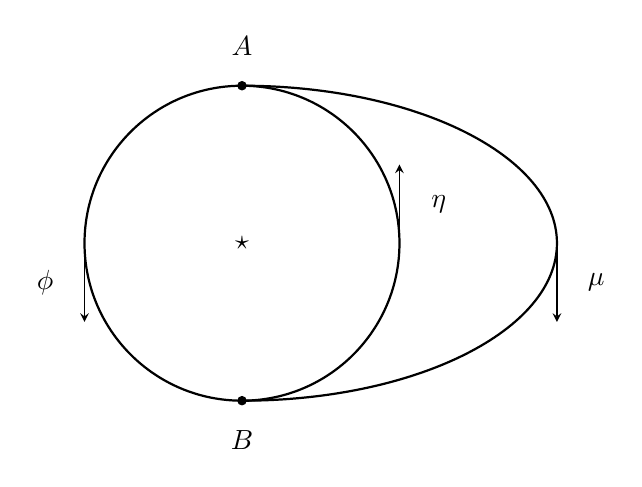
\begin{tikzpicture}
\draw[thick] (0,0) circle (2cm);
\draw (0,0) node {$\star$};

\draw[fill=black] (0,2) circle (1.5pt);
\draw (0,2.5) node {$A$};

\draw [-stealth] (2,0) -- (2,1);
\draw (2.5,0.5) node {$\eta$};

\draw[fill=black] (0,-2) circle (1.5pt);
\draw (0,-2.5) node {$B$};

\draw [-stealth] (-2,0) -- (-2,-1);
\draw (-2.5,-0.5) node {$\phi$};

%Primera distancia -> Eje horizontal
%Segunda distancia -> Eje vertical
\draw[thick] (0,2) arc (90:-90:4cm and 2cm);

\draw [-stealth] (4,0) -- (4,-1);
\draw (4.5,-0.5) node {$\mu$};
\end{tikzpicture}
}
	\caption{Varios caminos en $\mb{R}^2$.\labfig{MotivHomologia}}
\end{marginfigure}

Consieremos ahora el plano perforado, $X=\mb{R}^2\backslash\{(0,0)\}$.
La aplicación $\phi|_X+\eta|_X$ ya no forma el borde de una cadena singular, dado que los caminos encierran al punto $(0,0)$, que no está.
Por tanto, las clases de $\phi|_X$ y $\mu|_X$ serán diferentes.
En cambio, $\phi$ y $\psi$ siguen siendo homólogas, porque sus orientaciones son compatibles y no contienen al punto que hemos quitado.

Como consecuencia del \refthm{homologia invariante}, concluimos que $\mb{R}^2$ no es homeomorfo a $X$.

\subsection{Característica de Euler}
\marginnote[-2.2cm]{
\begin{kaobox}[frametitle=Rango de un grupo]
	Sea $A$ un grupo abeliano.
	Se denomina \textbf{subgrupo de torsión} de $A$ al subgrupo $T$ formado por todos los elementos de orden finito de $A$.
	Decimos que $A$ es \textbf{libre de torsión} si $T=0$, y que $A$ es un \textbf{grupo de torsión} si $T=A$.
	Definimos el \textbf{rango} de $A$ como el mínimo número de generadores que posee su subgrupo de torsión.
\end{kaobox}
}

\begin{example}
\begin{enumerate}
	\item El grupo aditivo $\mb{Z}_n=\mb{Z}/n\mb{Z}$ es un grupo de torsión: dado un $\overline{p} \in \mb{Z}_n$,
		\[n\overline{p}=\sum^{n|p|}_{i=1}\overline{1}=\sum^{|p|}_{i=1}\overline{n}=\sum^{|p|}_{i=1}0=0\]
	Por la misma razón, todo cuerpo de característica mayor que cero define un grupo de torsión.
	\item El grupo aditivo $\mb{Z}$ es un grupo libre de torsión porque no tiene divisores de cero: si $n > 0$ y $p \in \mb{Z}$ es tal que $np=0$, necesariamente se cumple que $p=0$.
	\item Consideramos $\mb{Z}\times \mb{Z}_n$: dado un $\overline{q} \in \mb{Z}_n$,
		\[n(0,\overline{q})=\sum^n_{i=1}(0,\overline{q})=(0,n\overline{q})=(0,0)\]
	por lo que el subgrupo de torsión de $\mb{Z}\times \mb{Z}_n$ contiene a $\{0\}\times\mb{Z}_n$.
	Sin embargo, si $m > 0$ y $p \in \mb{Z}$,
		\[m(p,\overline{q})=\sum^m_{i=1}(p,\overline{q})=(mp,m\overline{q})=(0,0)\]
	luego $n$ divide a $mq$ y $p=0$.
	Por tanto, el subgrupo de torsión de $\mb{Z}\times \mb{Z}_n$ es $\{0\}\times\mb{Z}_n$ (que es un subgrupo propio).
\end{enumerate}
\end{example}

\begin{definition}
Se define el \textbf{$n$-ésimo número de Betti} $\beta_n(X)$ como el rango de $H_n(X)$.
Si existe un $k \in \mb{N}$ tal que $\beta_p(X)=0$ para todo $p > k$, se define la \textbf{característica de Euler} de $X$ como 
	\[\chi(X):=\sum^k_{n=0}(-1)^n\beta_n(X)\]
\end{definition}
